\begin{figure}[t]
    \centering
    \begin{minipage}[t]{0.47\linewidth}
        \centering
        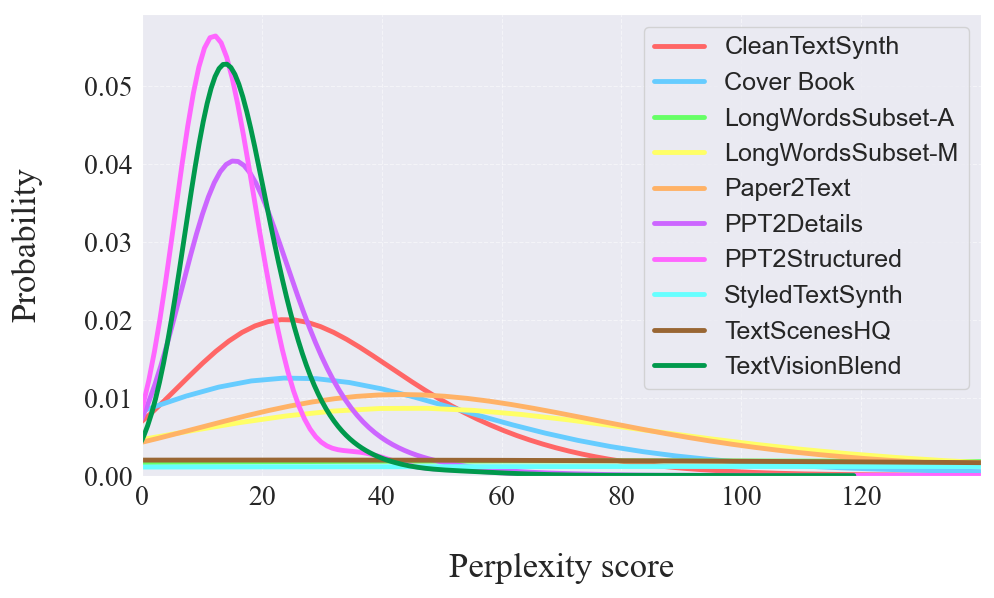
\includegraphics[width=\linewidth]{figures/src/perplexity.png}
        \caption*{\textbf{(a) Perplexity Distribution.} 
        Kernel density estimation comparing; lower perplexity indicates Wikipedia-like content.}
    \end{minipage}%
    \hfill
    \begin{minipage}[t]{0.52\linewidth}
        \centering
        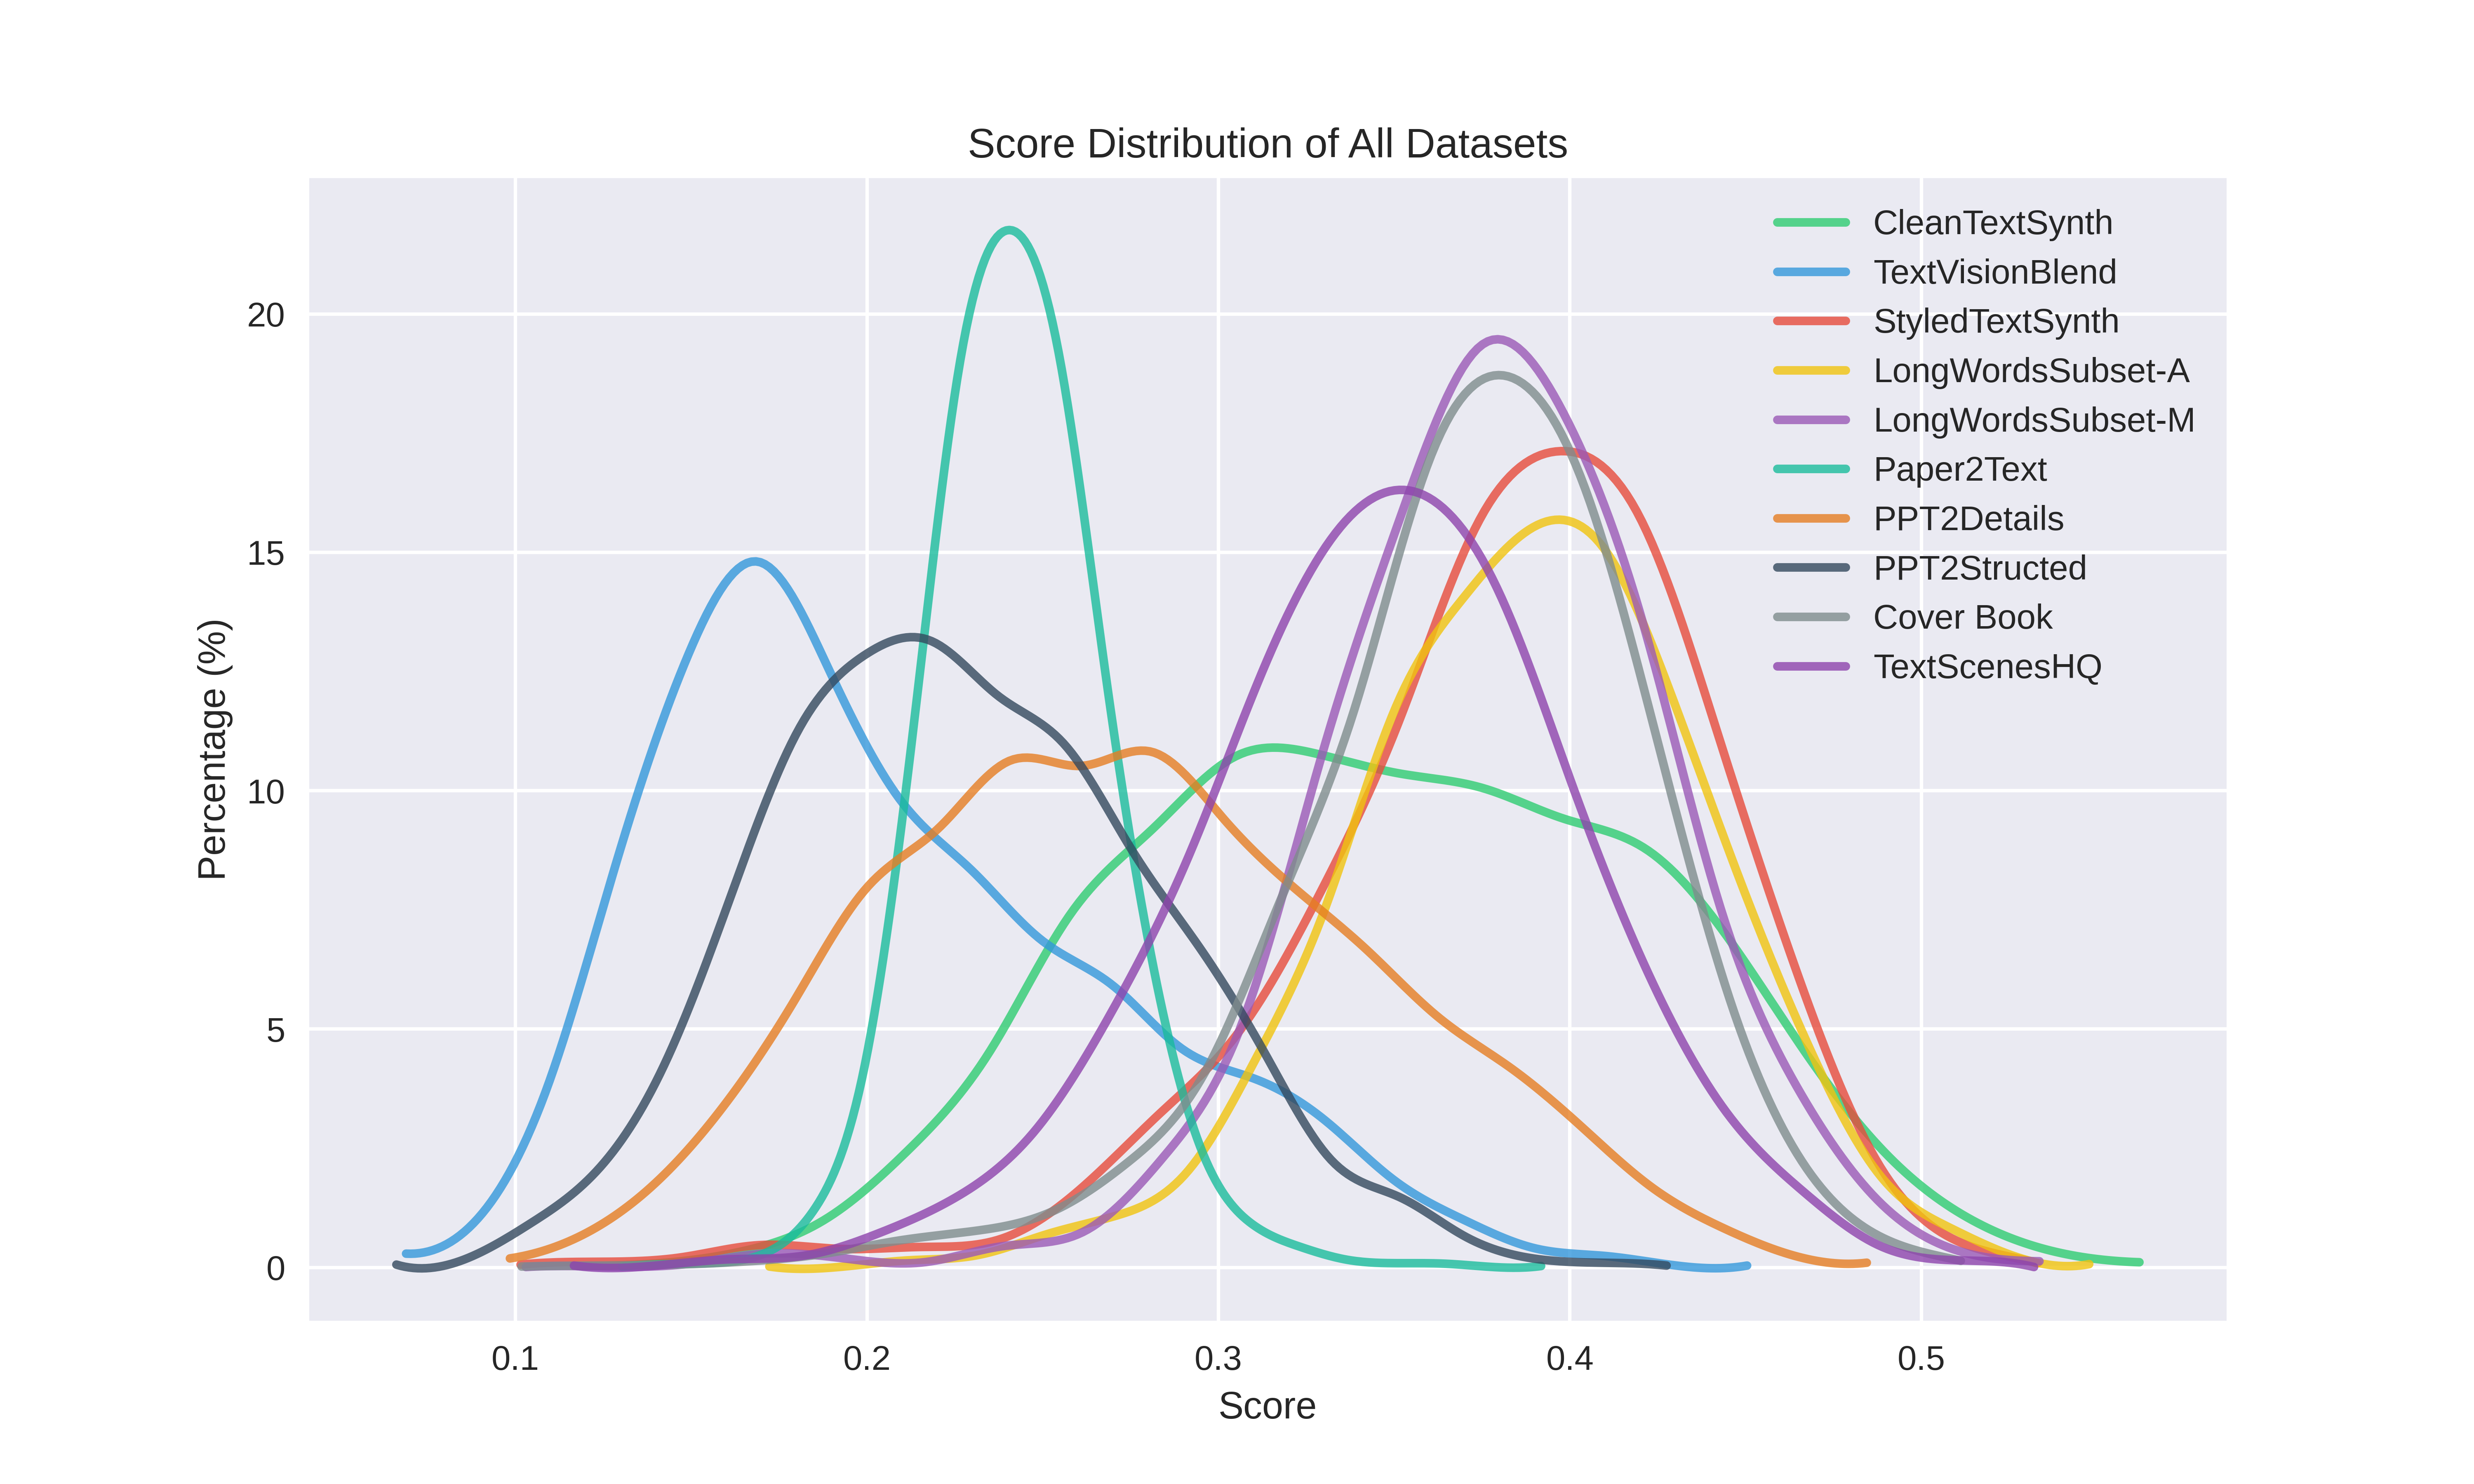
\includegraphics[width=\linewidth]{figures/src/clip_score.png}
        \caption*{\textbf{(b) CLIP Score Distribution.} 
        CLIP score distribution across all \DatasetName~subsets, using 10k random samples each.}
    \end{minipage}
    \caption{\textbf{Linguistic and Visual Quality of \DatasetName.} 
    (a) shows the perplexity distribution of text content, assessing linguistic quality. 
    (b) presents visual-text alignment across subsets.}
    \label{fig:quality_metrics}
\end{figure}


% \begin{figure}[t]
%     \centering
%     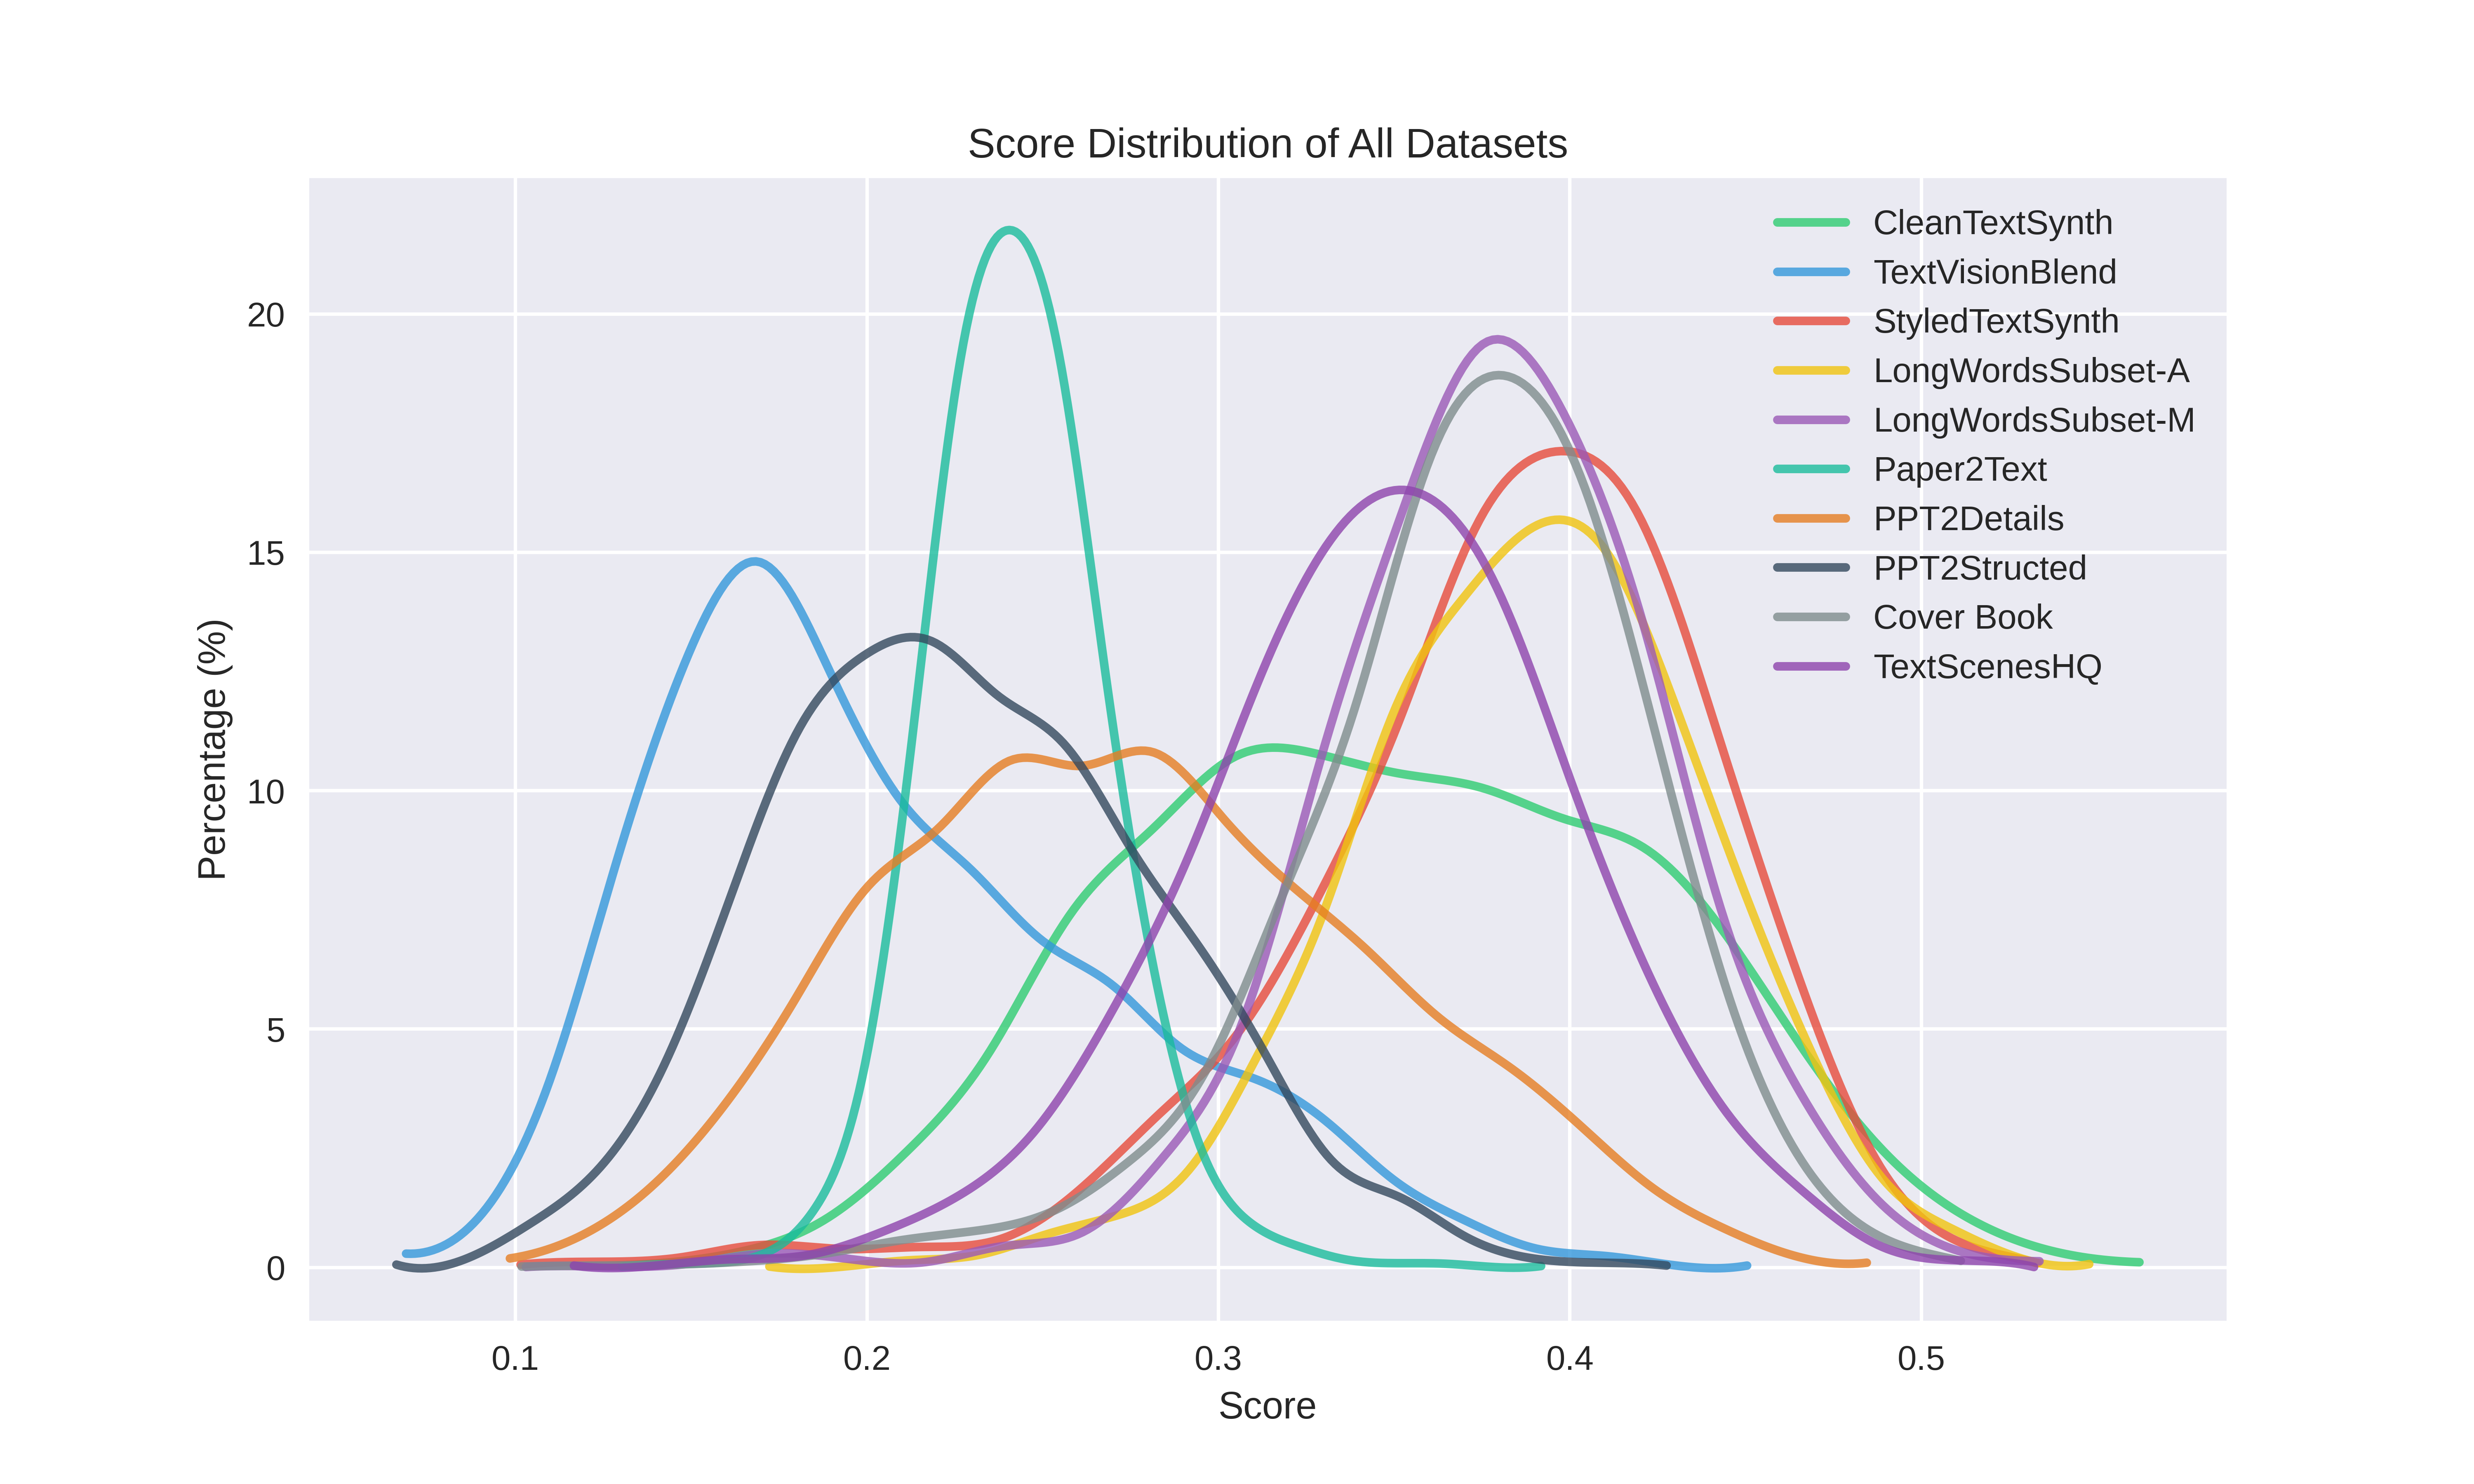
\includegraphics[width=\linewidth]{figures/src/clip_score.png}
%     \caption{
%     \textbf{Clip score distribution over all sub datasets in \DatasetName}.
%     We randomly sample 10k samples for each subset in \DatasetName.
%     }
%     \label{fig:clip score subdataset}
% \end{figure}